% Carattere dimensione 12
\documentclass[11pt,openany]{report}

\setlength{\parindent}{0pt}

% Per la stampa fronte-retro sostituire con:
% \documentclass[12pt, twoside]{report}

% Margini (4cm a sx, 2.5cm a dx, 2.5cm in alto, 2.5cm in basso)
\usepackage[top=2cm, bottom=2cm, left=1.5cm, right=1.5cm, centering]{geometry}

% Per la stampa fronte-retro sostituire con: 
% \usepackage[top=2.5cm, bottom=2.5cm, inner=4cm, outer=4cm, right=2.5cm, centering]{geometry}

% Interlinea
\linespread{1.2}

\usepackage{booktabs}

% Librerie utili
\usepackage[english]{babel} % applicazione regole di scrittura per la lingua italiana 
\usepackage[utf8]{inputenc} % codifica UTF-8
\usepackage{scrlayer-scrpage} % stili pagina per il frontespizio
\ifoot[]{}
\cfoot[]{}
\cfoot[\pagemark]{\pagemark}
\pagestyle{scrplain}
\usepackage{lmodern} % font Times New Roman (simile)
\usepackage{graphicx} % inserimento di immagini
\usepackage{subcaption}
\usepackage{csquotes} % per le citazioni "in blocco"
\usepackage[backend=biber, sorting=none, ]{biblatex} % bibliografia con pacchetto biblatex (https://ctan.org/pkg/biblatex?lang=en)
\addbibresource{bibliography.bib}
\appto{\bibsetup}{\raggedright}


\usepackage{titlesec} % per la formattazione dei titoli delle sezioni, capitoli etc.
\usepackage{float} % per il posizionamento delle immagini

\usepackage{listings} % per il codice di programmazione
% Fonte https://en.wikibooks.org/wiki/LaTeX/Source_Code_Listings. Per la lista di sintassi riconosciute.
\renewcommand{\lstlistingname}{Code}% Listing -> Codice
\usepackage{xcolor}  % stile del codice
\definecolor{mygreen}{rgb}{0,0.6,0}
\definecolor{mygray}{rgb}{0.5,0.5,0.5}
\definecolor{mymauve}{rgb}{0.58,0,0.82}
\definecolor{darkgray}{rgb}{.4,.4,.4}
\definecolor{navy}{HTML}{000080}
\definecolor{purple}{rgb}{0.65, 0.12, 0.82}
\definecolor{codepurple}{rgb}{0.58,0,0.82}
\definecolor{backcolour}{rgb}{0.95,0.95,0.92}

% \usepackage{longtable}
\usepackage{tabularx}
\usepackage{ragged2e}
\usepackage{multicol} % Per supportare colonne multiple




% Stili configurabili del codice (lslisting) 
\lstset{ %
belowcaptionskip=0.5em,
backgroundcolor=\color{backcolour}, % choose the background color; you must add \usepackage{color} or \usepackage{xcolor}
basicstyle=\footnotesize, % the size of the fonts that are used for the code
breakatwhitespace=false, % sets if automatic breaks should only happen at whitespace
breaklines=true, % sets automatic line breaking
captionpos=b, % sets the caption-position to bottom
commentstyle=\color{mygreen}, % comment style
deletekeywords={...}, % if you want to delete keywords from the given language
escapeinside={\%*}{*)}, % if you want to add LaTeX within your code
extendedchars=true, % lets you use non-ASCII characters; for 8-bits encodings only, does not work with UTF-8
frame=single, % adds a frame around the code
keepspaces=true, % keeps spaces in text, useful for keeping indentation of code (possibly needs columns=flexible)
keywordstyle=\color{codepurple}, % keyword style
% language=Octave, % the language of the code
morekeywords={*,...}, % if you want to add more keywords to the set
numbers=left, % where to put the line-numbers; possible values are (none, left, right)
numbersep=5pt, % how far the line-numbers are from the code
numberstyle=\tiny\color{mygray}, % the style that is used for the line-numbers
rulecolor=\color{black}, % if not set, the frame-color may be changed on line-breaks within not-black text (e.g. comments (green here))
showspaces=false, % show spaces everywhere adding particular underscores; it overrides 'showstringspaces'
showstringspaces=false, % underline spaces within strings only
showtabs=false, % show tabs within strings adding particular underscores
stepnumber=1, % the step between two line-numbers. If it's 1, each line will be numbered
stringstyle=\color{mymauve}, % string literal style
tabsize=2, % sets default tabsize to 2 spaces
title=\lstname % show the filename of files included with \lstinputlisting; also try caption instead of title
}


% Formato delle intestazioni
% \titleformat{\chapter}[hang]{\normalfont\Large\bfseries}{\thechapter.}{0.5em}{}


\makeatletter
\renewcommand{\chapter}{\@startsection{chapter}{0}{0pt}
  {-7ex plus -1ex minus -.2ex}
  {2ex plus .2ex}
  {\normalfont\Large\bfseries}}
\makeatother

% \titlespacing*{\chapter}{0pt}{3em}{1.5em}


\titleformat{\chapter}[hang]          % no "Chapter", just number and title
  {\normalfont\Large\bfseries}       % formatting of the whole line
  {\thechapter.}                     % numbered like "1."
  {0.5em}                            % spacing between number and title
  {}                                 % what to put before the title text

\titlespacing*{\chapter}             % controls vertical spacing
  {0pt}                              % left margin
  {3em}                              % space *before* chapter title
  {1.5em} 


% % Prevent chapters from starting on a new page
% \makeatletter
% \renewcommand{\@makechapterhead}[1]{%
%   {\parindent \z@ \raggedright \normalfont
%   \interlinepenalty\@M
%   \Huge\bfseries \thechapter. #1\par\nobreak
%   \vskip 20pt }}
% \makeatother

% % Optional: If you also want unnumbered chapters to not start on a new page:
% \makeatletter
% \renewcommand{\@makeschapterhead}[1]{%
%   {\parindent \z@ \raggedright
%   \normalfont
%   \Huge\bfseries #1\par\nobreak
%   \vskip 20pt }}
% \makeatother

% % Chapter format: no "Chapter" word, just "1. Title"
% \titleformat{\chapter}[hang]
%   {\normalfont\Large\bfseries}
%   {\thechapter.}
%   {0.5em}
%   {}

% % Spacing: left indent, before title, after title
% \titlespacing*{\chapter}
%   {0pt}
%   {5em}  % space *before* title
%   {2em}  % space *after* title


\begin{document}


% Frontespizio
% \begin{titlepage}
% \begin{figure}
%     \centering
\includegraphics[scale=0.5]{immagini/cherubino_pant541.png}
% \end{figure}
\pagestyle{empty}         % niente numero di pagina
\pagenumbering{gobble}    % disattiva numerazione
\begin{center}  
     {\LARGE { Data Mining: Fundamentals}}\\
     \vspace{2cm}
    {\Large { A.Y. 2024/2025 }}\\
    \vspace{2cm}
    {\Large { Group 12 }}\\
     \vspace{2cm}
     {\large { Bruno Barbieri, Noemi Dalmasso, Gaia Federica Francesca Ferrara }}
\end{center}

The aim of this report is to display an analysis carried out on the IMDb dataset; the analysis has been conducted making use of data mining methodologies. 
After the data understanding and preparation phase, clustering, classification, regression and pattern mining techniques have been applied.

% \vspace{2cm}

% \begin{minipage}[t]{0.47\textwidth}
%   {\large{\bf Relatore:\\ Nome Cognome}}
% 	\vspace{0.5cm}
% 	{\large{\bf \\Correlatore:\\ Nome Cognome}}
% \end{minipage}\hfill\begin{minipage}[t]{0.47\textwidth}\raggedleft
%   {\large{\bf Group 12\\ }}
%   \vspace{0.5cm}
  
% \end{minipage}

% \vspace{25mm}

% \centering{\large{\bf ANNO ACCADEMICO 20xx/20xx }}
% \end{titlepage}
% Fine frontespizio
\clearpage

\tableofcontents
\clearpage

\pagenumbering{arabic}  % numerazione araba
\setcounter{page}{1}    % riparti da pagina 1
\pagestyle{scrplain}    % stile pagina con numeri al centr

% \addtocontents{toc}{\protect\thispagestyle{empty}}
% \addcontentsline{toc}{chapter}{Introduction} % Capitolo non numerato
%\chapter*{Introduzione}
\label{ch:introduzione}

Introduzione...


\chapter{Data Understanding and Preparation}
\label{ch:capitolo1}

% --- Inizio del Capitolo 1 ---

% Capitolo 1...

% Esempio di una nota\footnote{CleanCode} con citazione a sezione~\ref{sec:sezione1}.

% \begin{figure}[H]
%     \centering
%     
\includegraphics[width=0.2\textwidth]{immagini/logo-dip_blu_hr.png}
%     \caption{Esempio di un'immagine}
%     \label{fig:immagine1}
% \end{figure}

% \begin{lstlisting}[caption={Esempio codice JavaScript},label={Esempio codice JavaScript}, language=JavaScript]
% function foo(num) {
%     const bar = 2;
%     return num + bar;
% }

% const result = foo(2);
% // result -> 4
% \end{lstlisting}


% \section{Sezione 1}\label{sec:sezione1}


% Sezione 1... con citazione bibliografica~\cite{CleanCode}

% \subsection{Sottosezione 1}
% \label{subsec:sottosezione1}

% Sottosezione 1...

\section{Data Semantics}\label{sec:data_semantics}
The dataset \textit{complete\_df.csv}, which is the merge of the original \textit{train.csv} and \textit{test.csv} datasets, contains 21909 titles of different forms of visual entertainment that have been rated on IMDb, an online database of information related to films, television series etc. 
Each record is described by 23 attributes, both numerical and non-numerical. 
All the variables of the dataset are introduced and explained in Table 1.1 and Table 1.2.
\begin{table}[h]
    \centering
    \begin{tabular}{|l|l|l|} % Using 'l' for left alignment of columns
        \hline
        \textbf{Attribute} & \textbf{Type} & \textbf{Description} \\ 
        \hline
        originalTitle & Nominal & Title in its original language \\  
        \hline
        rating & Ordinal & IMDB title rating class \\
        & & The range is from (0,1] to (9,10] \\ 
        \hline
        titleType & Nominal & The format of the title \\ 
        \hline
        canHaveEpisodes & Nominal (Binary) & Whether or not the title can have episodes \\ 
        & & True: can have episodes; False: cannot have episodes \\ 
        \hline
        isRatable & Nominal (Binary) & Whether or not the title can be rated by users \\ 
        & & True: it can be rated; False: cannot be rated \\ 
        \hline
        isAdult & Nominal (Binary) & Whether or not the title is for adults \\ 
        & & 0: non-adult title; 1: adult title \\ 
        \hline
        countryOfOrigin & Nominal & The country(ies) where the title was produced \\ 
        \hline
        genres & Nominal & The genre(s) associated with the title \\ 
        \hline
    \end{tabular}
    \caption{Description of non-numerical attributes}
    \label{tab:attributes}
\end{table}
\begin{table}[h]
    \centering
    \begin{tabular}{|l|l|l|} % Using 'l' for left alignment of columns
        \hline
        \textbf{Attribute} & \textbf{Type} & \textbf{Description} \\ 
        \hline
        runtimeMinutes & Numeric & Runtime of the title expressed in minutes \\ 
        \hline
        startYear & Interval & Release/start year of a title \\ 
        \hline
        endYear & Interval & TV Series end year \\
        \hline
        awardWins & Numeric & Number of awards the title won \\ 
        \hline
        numVotes & Numeric & Number of votes the title has received \\ 
        \hline
        worstRating & Numeric & Worst title rating \\ 
        \hline
        bestRating & Numeric & Best title rating \\ 
        \hline
        totalImages & Numeric & Number of Images on the IMDb title page \\ 
        \hline
        totalVideos & Numeric & Number of Videos on the IMDb title page \\ 
        \hline
        totalCredits & Numeric & Number of Credits for the title \\ 
        \hline
        criticReviewsTotal & Numeric & Total Number of Critic Reviews \\ 
        \hline
        awardNominationsExcludeWins & Numeric & Number of award nominations excluding wins \\ 
        \hline
        numRegions & Numeric & The regions number for this version of the title \\ 
        \hline
        userReviewsTotal & Numeric & Number of User Reviews \\ 
        \hline
        ratingCount & Numeric & The total number of user ratings for the title \\ 
        \hline
    \end{tabular}
    \caption{Description of numerical attributes}
    \label{tab:numerical_attributes}
\end{table}
\section{Distribution of the variables and statistics}\label{sec:variable_distrib}
\subsection{Discrete attributes}
In this paragraph, we examine the most informative discrete attributes of the dataset to provide an overview of their statistics and frequencies. 
\\From Fig.1.1(a), we observe that the classes of the \textit{titleType} attribute are unbalanced, with \textit{movie} being the most frequent class (5535 records) and \textit{tvShort} the least frequent (40 records). By analyzing the \textit{canHaveEpisodes} attribute within these \textit{titleType} values, we found out that only \textit{tvSeries} and \textit{tvMiniSeries} can have episodes, as expected.
\\As shown in Fig.1.1(b), the frequency of rating classes is skewed toward higher values. The most frequent rating class is (7, 8], which is the rating of 4822 titles.
\\Another important aspect is that all 16341 titles are ratable and the vast majority of them (16005) are non-adults contents, as shown in Fig.1.1(c)
\begin{figure}[h!]
    \centering
    \subfigure[(a)]{
        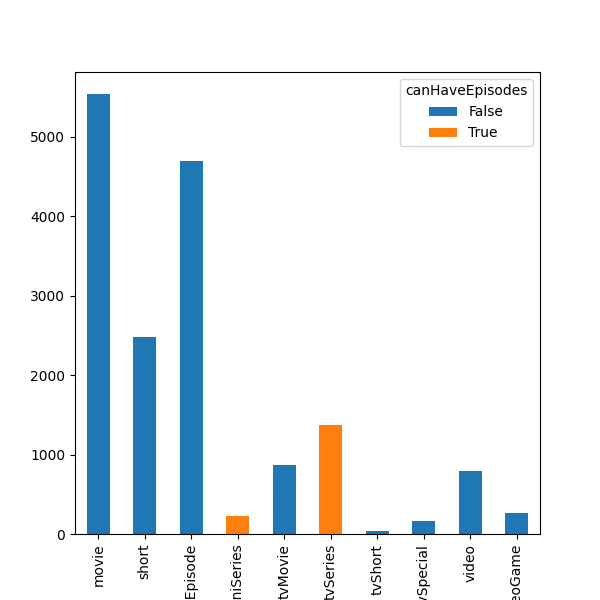
\includegraphics[width=0.45\textwidth]{plots/fig1_a.png} % Replace with your plot
        }
    \subfigure[(b)]{
        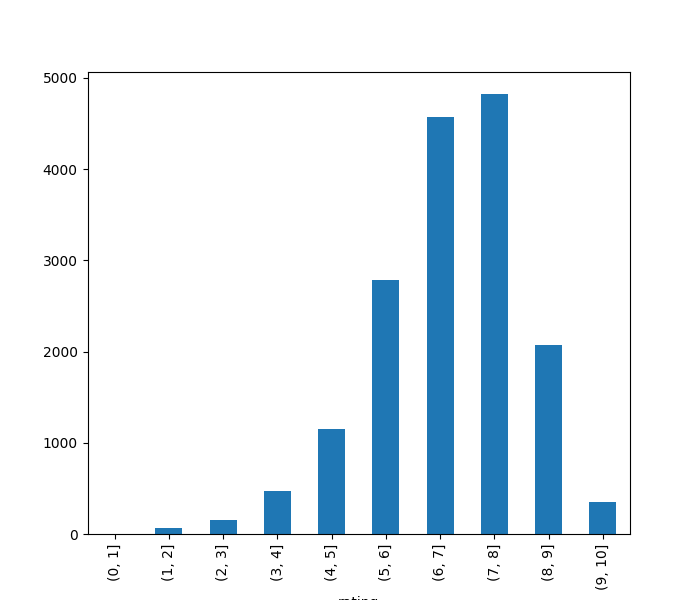
\includegraphics[width=0.45\textwidth]{plots/fig1_b.png}
        }
    \subfigure[(c)]{
        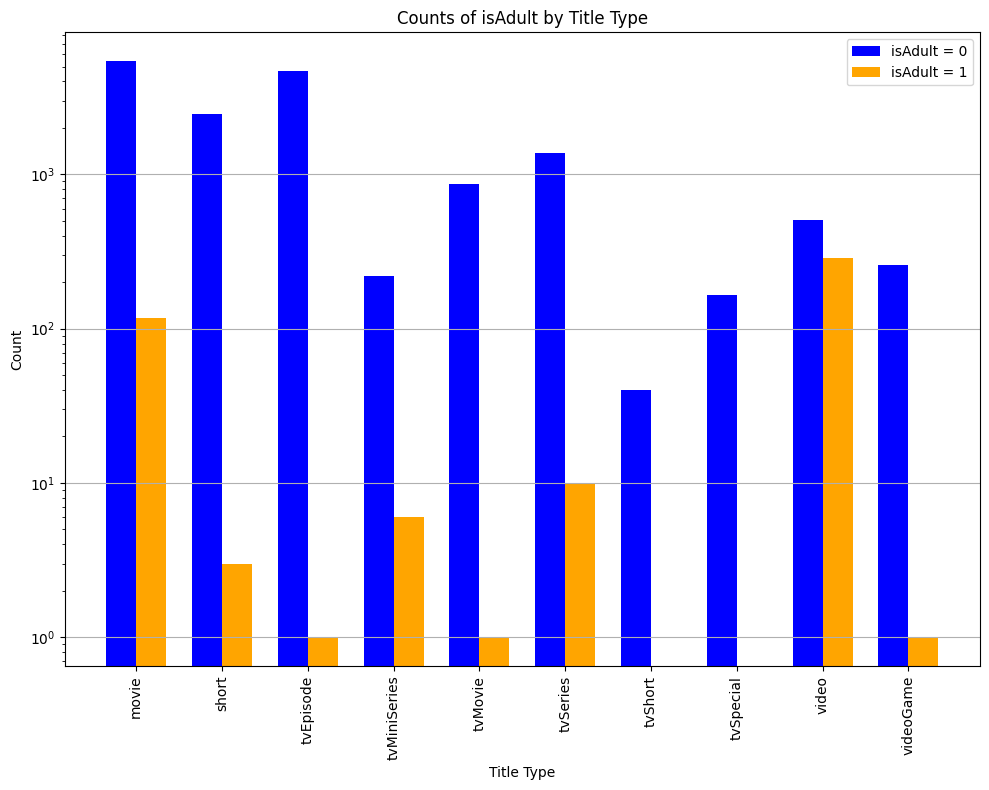
\includegraphics[width=0.45\textwidth]{plots/fig1_c.png}
        }
    \caption{Bar chart of the discrete attributes: (a): counting of the title types frequencies combined with the canHaveEpisodes variable (b): counting of ratings frequencies (c): counting of the adult and non-adult frequencies combined with the isRatable attribute.}
    \label{fig:bar-charts}
\end{figure}
\subsection{Continuous attributes}
...content...
...content...
...content...
...content...
...content...
...content...
...content...
...content...
...content...
...content...


\end{document}
 %data preparation

\chapter{Clustering}
\label{ch:capitolo2}

This chapter of the report aims at illustrating the clustering analysis performed on the dataset at hand.
The employed clustering techniques are K-means (Centroid-based), DBSCAN (density-based) and hierarchical clustering.

The analysis conducted using these methods focused only exclusively on the dataset's numerical attributes, which were appropriately log-transformed (as mentioned in the \textit{Variable Transformation} section) and normalized using \texttt{MinMaxScaler}.  
For the K-means algorithm, \texttt{totalNominations} and \texttt{totalMedia} were excluded due to their high proportion of zero values, which negatively affected cluster formation.

In addition, an attempt was made to incorporate categorical variables to the analysis with the K-means algorithm by converting them into binary attributes and constructing a mixed-distances matrix. 
Distances were then calculated using the Euclidean distance for numerical (log-tranformed and scaled) features and the Jaccard similarity for binary ones. 
However, this approach was computationally expensive and did not lead to any improvement in the results.

\textbf{RIVEDERE PARTE PCA}
Principal Component Analysis (PCA) was applied to the preprocessed data just for clusters visualization purposes. 
Analysis of the numerical attributes reveals that 4 principal components are optimal when excluding variables with many zero values, while 5 components are needed when including all variables. 
These numbers of components capture the maximum meaningful variance, as shown by the point in the plots where where the line starts to flatten, indicating that adding more components doesn't increase explained variance significantly. 
The plots in figure~\ref{fig:pca_diff} show the differences between these two approaches. \textbf{IN REALTA' NON SI VEDE TROPPO LA DIFFERENZA, QUINDI MAGARI NON FARE PCA MA SOLO VISUALIZZAZIONE CON ISTOGRAMMI??? oppure semplicemente tenere solo uno dei due plot?}
\begin{figure}[H]
    \centering
    \begin{subfigure}[b]{0.40\textwidth}
        \centering
        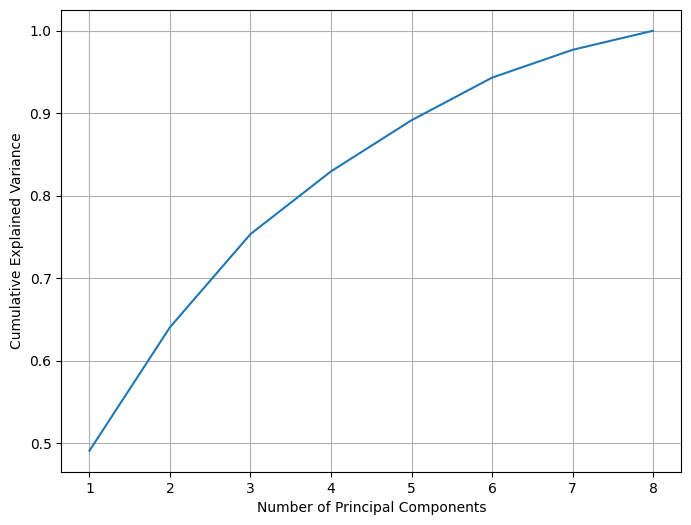
\includegraphics[width=\textwidth]{plots/pca_kmeans.png}
        \caption{PCA excluding variables}
        \label{fig:sse_silh_kmeans}
    \end{subfigure}
    \begin{subfigure}[b]{0.40\textwidth}
        \centering
        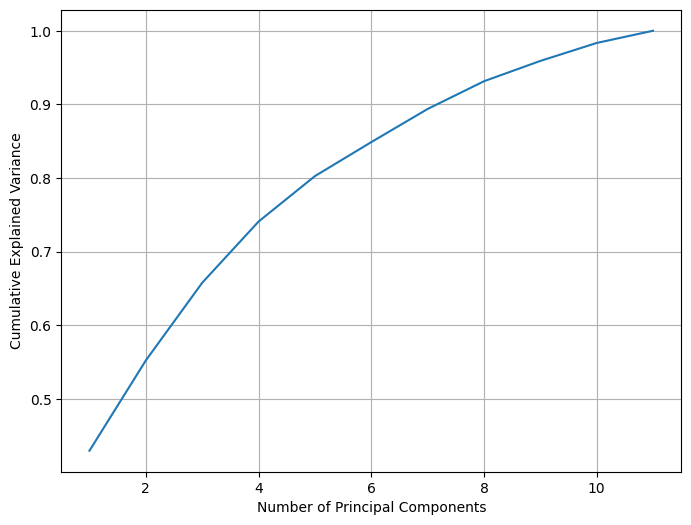
\includegraphics[width=\textwidth]{plots/pca5.png}
        \caption{PCA with all variables}
        \label{fig:pca5}
    \end{subfigure}
    \caption{Principal Component Analysis}
    \label{fig:pca_diff}
\end{figure}

\section{K-means}\label{sec:centroid_based}
%The clustering analysis performed with the K-means algorithm focused on the numeric variables of the dataset, excluding \texttt{awardWins}, \texttt{awardNominationsExcludeWins}, and \texttt{totalCredits} due to their high proportion of zero values, which negatively affected cluster formation. 
%The variables have been appropriately log-transformed (as illustrated in the \textit{Variable Transformation} section) and normalized with \texttt{StandardScaler}.

To identify the optimal number of clusters, both the SSE and Silhouette scores were computed. The goal was to find a configuration that minimizes the SSE while maintaining a robust Silhouette score and a proper \textit{k}. 
The plots in figure~\ref{fig:sse_silh_kmeans} demonstrate that \textit{k} = ??? provides the optimal balance between these metrics. Choosing \textit{k} = ??? returns a SSE score of ??? and Silhouette score of ???. 
\textbf{VALORI TROPPO ALTI, VEDERE SE CAMBIANO CAMBIANDO SCALING E/O TOGLIENDO OUTLIER}

% To visualize the clustering results, Principal Component Analysis (PCA) was employed. The plot in figure~\ref{fig:pca_kmeans} reveals that 4 principal components are enough to capture the optimal amount of variance for the selected variables, as evidenced by the the point where the line starts to flatten, indicating that adding more components doesn't increase explained variance significantly.
The cluster results are presented in figure~\ref{fig:pairplot_kmeans}. 

\begin{figure}[H]
    \centering
    \begin{subfigure}[b]{0.49\textwidth}
        \centering
        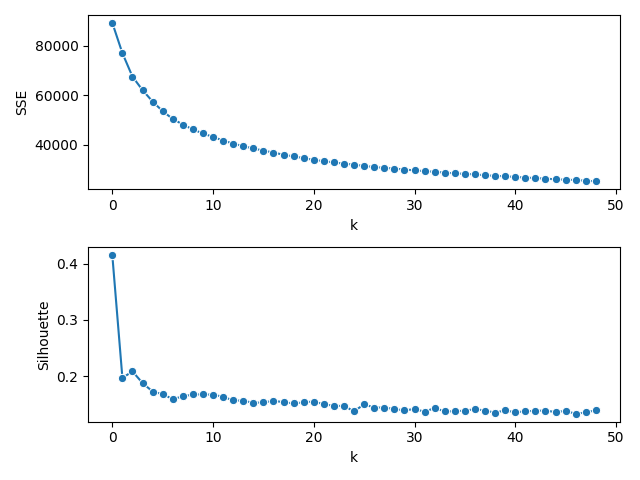
\includegraphics[width=\textwidth]{plots/sse_silh_kmeans.png}
        \caption{SSE and Silhouette scores}
        \label{fig:sse_silh_kmeans}
    \end{subfigure}
    % \hfill
    % \begin{subfigure}[b]{0.3\textwidth}
    %     \centering
    %     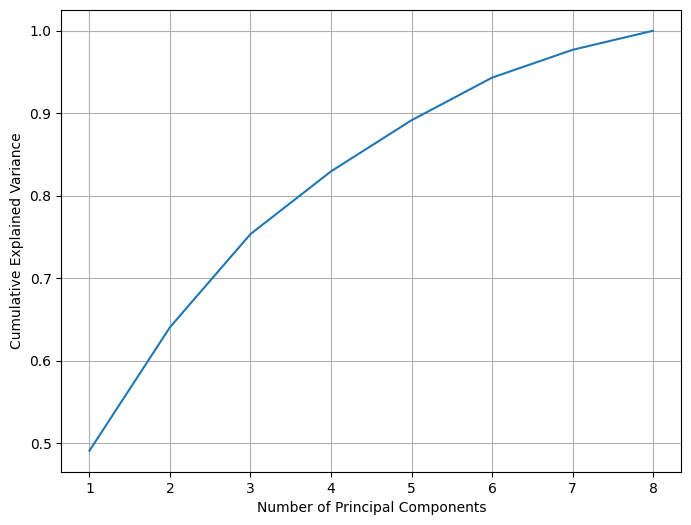
\includegraphics[width=\textwidth]{plots/pca_kmeans.png}
    %     \caption{PCA Analysis}
    %     \label{fig:pca_kmeans}
    % \end{subfigure}
    % \hfill
    \begin{subfigure}[b]{0.49\textwidth}
        \centering
        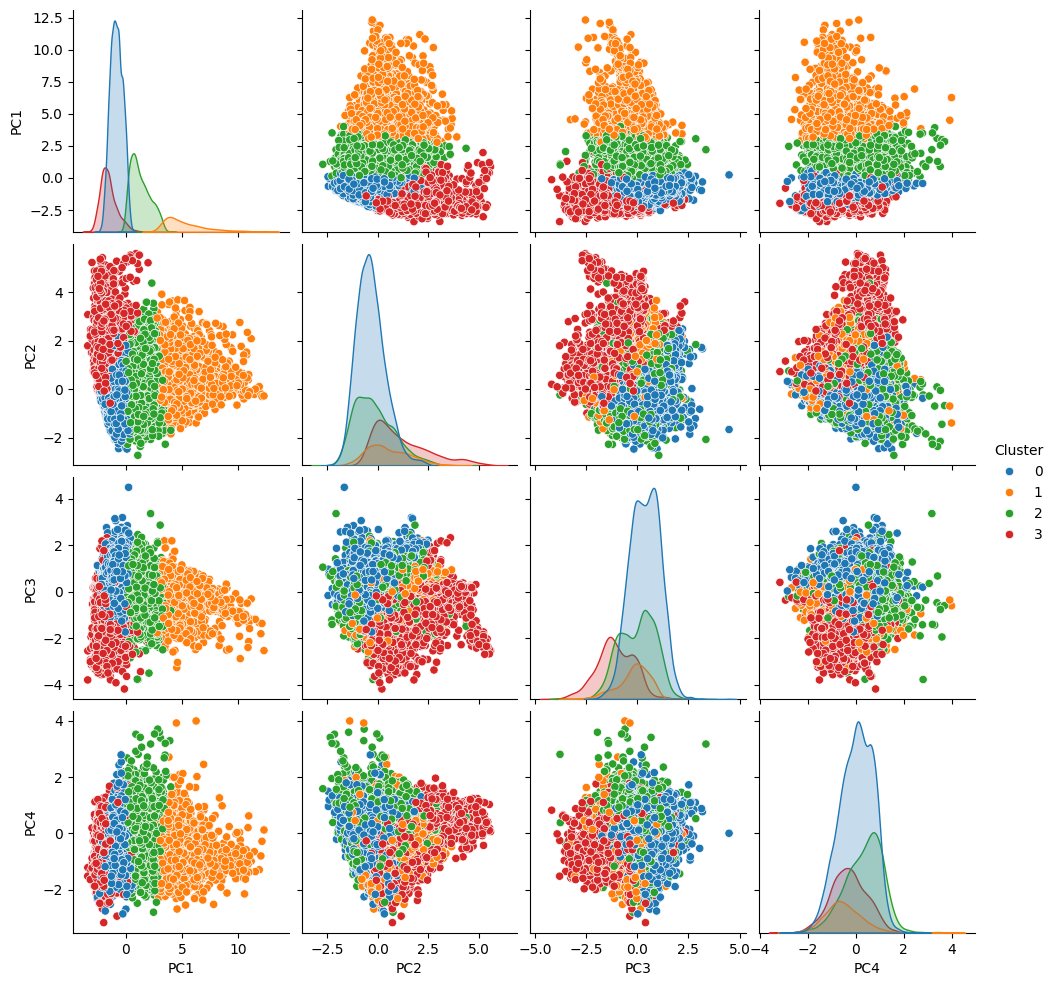
\includegraphics[width=\textwidth]{plots/pairplot_kmeans.png}
        \caption{K-means Visualization}
        \label{fig:pairplot_kmeans}
    \end{subfigure}
    \caption{K-means clustering analysis}
    \label{fig:three_subplots}
\end{figure}
The distribution of data points across the four clusters is as follows (shown in percentage of data points per cluster):
% Red (0): 51.68\%, Blue (1): 7.42\%, Green (2): 24.22\%, Orange (3): 16.68\%.
% The clusters are not as well-separated in most Principal Component combinations as they are with PC1. 
% In fact, in the other combinations, the clusters tend to overlap and their boundaries are not always clearly distinct.
% This might be an indication that the true clusters have irregular shapes or different densities, resulting in boundaries between them being not clearly defined.



\section{DBSCAN}\label{sec:density_based}
To determine the optimal DBSCAN parameters, the \textit{k\textsuperscript{th} nearest neighbors} method was used: this allows to identify \textit{eps} (the maximum distance between two points for them to be considered neighbors) given the value of \textit{Minpts} (minimum number of points in a neighborhood for a point to be considered a core point).
Initially, \textit{Minpts} was set to 22, following the rule of setting it above twice the number of dimensions. 
However, due to the dataset's unbalanced nature and the sparsity of high-dimensional data, reducing \textit{Minpts} to 11 allowed the formation of smaller clusters while preventing the risk of detecting only one dominant cluster and classifying many minority groups as noise instead of distinct clusters.
To determine \textit{eps}, the k\textsuperscript{th} nearest neighbors plot with \textit{k} = 11 was analyzed (figure ~\ref{fig:DBSCAN_kth_graph}). While the "knee" point suggested an eps of around 0.1, this value would have resulted in excessive noise and a single dominant cluster. 
To address this, eps was set to 1.564, allowing for meaningful connectivity while preserving the detection of smaller clusters without merging them into a single entity. 
The algorithm identified 4 groups in the dataset, including one representing noise (1,753 points). 
The largest cluster contains 13,198 points, while the smaller clusters consist of 733 and 747 points, 
respectively.The  results are shown in figure~\ref{fig:DBSCAN_provvisoria}

To conclude, by adjusting \textit{eps} and \textit{Minpts} appropriately, the clustering results achieved a Silhouette score of 0.139 \textbf{(SIL CONTANDO OUTLIERS)}, indicating little improved cluster separation and reduced noise, which is considered good enough for an unbalanced, high-dimensional dataset.

\begin{figure}[H]
    \centering
    \begin{subfigure}[b]{0.49\textwidth}
        \centering
        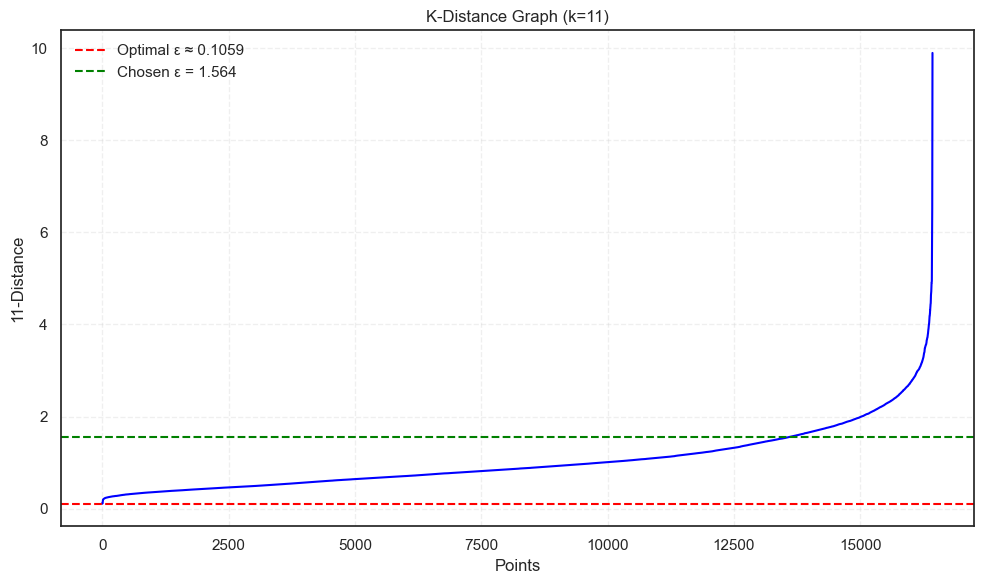
\includegraphics[width=\textwidth]{plots/DBSCAN_kth_graph.png}
        \caption{k\textsuperscript{th} nearest neighbors}
        \label{fig:DBSCAN_kth_graph}
    \end{subfigure}
    % \hfill
    % \begin{subfigure}[b]{0.3\textwidth}
    %     \centering
    %     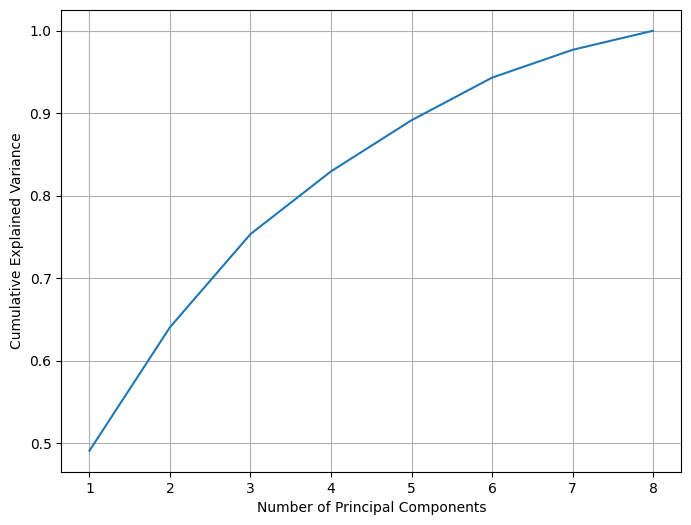
\includegraphics[width=\textwidth]{plots/pca_kmeans.png}
    %     \caption{PCA Analysis}
    %     \label{fig:pca_kmeans}
    % \end{subfigure}
    % \hfill
    \begin{subfigure}[b]{0.49\textwidth}
        \centering
        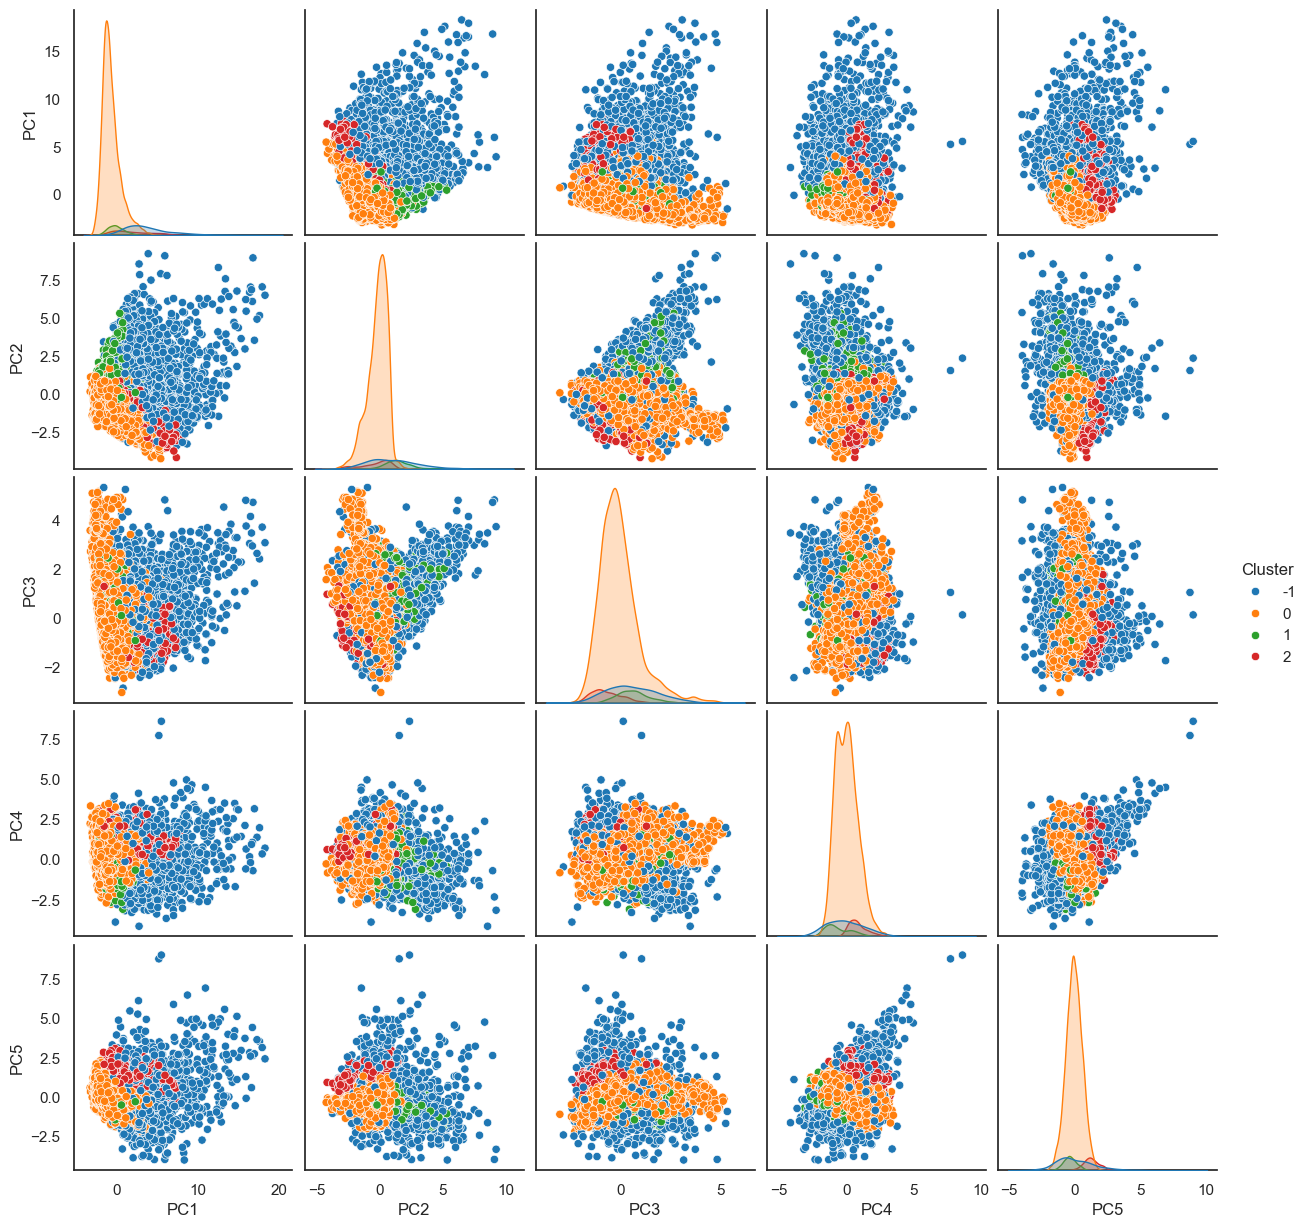
\includegraphics[width=\textwidth]{plots/DBSCAN_provvisoria.png}
        \caption{DBSCAN Visualization}
        \label{fig:DBSCAN_provvisoria}
    \end{subfigure}
    \caption{DBSCAN clustering analysis}
    \label{fig:three_subplots}
\end{figure}




\section{Hierarchical clustering}\label{sec:hierarchical}
Hierarchical clustering was performed using all linkages (Ward, Average, Complete, Single), with the Euclidean distance metric.
Figure~\ref{fig:hier_clust_stats} shows the results of the analysis, which includes the Silhouette and SSE scores, as well as the maximum and minimum percentage of points per cluster.
\begin{figure}[H]
    \centering

    % Left: Tall figure (a)
    \begin{subfigure}[t]{0.49\textwidth}
        \centering
        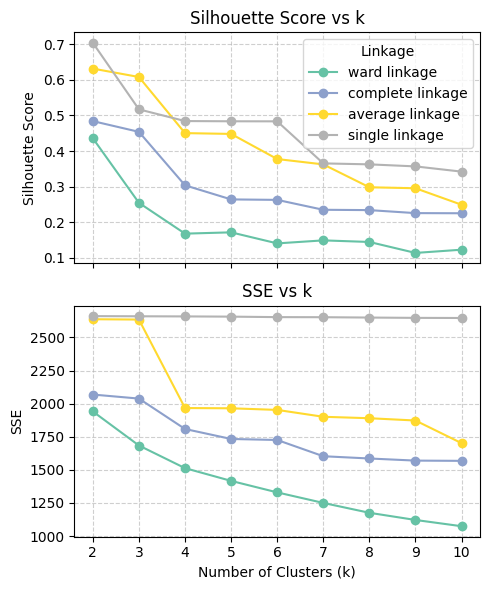
\includegraphics[width=0.95\textwidth]{plots/sil_sse_hierarchical_clust.png}
        \subcaption{Silhouette and SSE scores}
        \label{fig:sil_sse_hierarchical_clust}
    \end{subfigure}
    \hfill
    \begin{subfigure}[t]{0.49\textwidth}
        \centering
        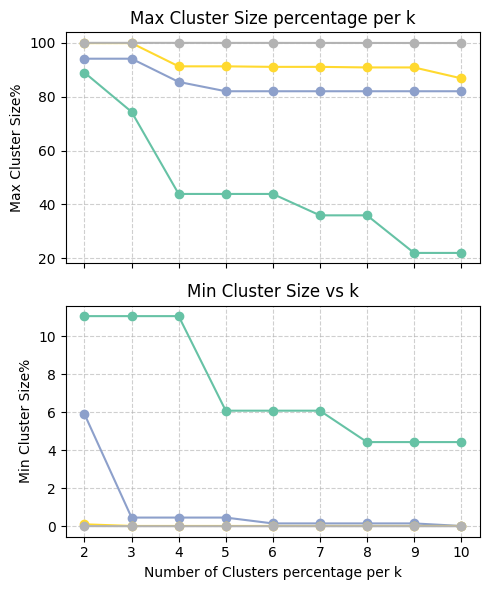
\includegraphics[width=0.95\textwidth]{plots/max_min_pctg.png}
        \subcaption{Max/Min percentage of points per cluster}
        \label{fig:max_min_pctg}
    \end{subfigure}
    \caption{Hierarchical clustering metrics for different numbers of clusters}
    \label{fig:hier_clust_stats}
\end{figure}

From figure~\ref{fig:max_min_pctg}, it can be observed that Single linkage produces a single cluster which contains basically all data points. This makes it unsuitable for this use case.
Average and Complete linkages produce a cluster with a high maximum cluster size (above 90\% of the dataset for all the number of clusters tested for Average, and 80\% for Complete).
These results are likely due to a few different causes: 
\begin{itemize}
    \item High density of points in a certain area of the feature space, which leads to the formation of large clusters;
    \item Presence of outliers (other than the ones that were removed), which can skew the clustering results by pulling the centroids towards them, resulting in larger clusters;
    \item High dimensionality of the dataset, which makes it more difficult to separate clusters effectively.
\end{itemize}

These issues are mitigated by Ward linkage, which produces less dominant biggest clusters for all numbers of clusters tested. The minimum cluster size is also consistently more balanced across different numbers of clusters.


\section{General considerations}\label{sec:considerations} %clustering


\chapter{Classification}
\label{ch:capitolo3}
Classification was performed on the available training set using three different algorithms: K-NN (\textit{K-Nearest Neighbours}), Naïve Bayes and Decision Trees.
For K-NN \textbf{and Naïve Bayes}, a portion of the training set (referred to as the validation set) was used to select the best hyperparameters \textbf{each} model.
The features used in K-NN and Naïve Bayes were normalized, as these models are sensitive to unscaled values.
In particular, a log-transformation and \textbf{SCRIVERE SE StandardScaler O MINMAX} were applied to data.
After training, the models were evaluated on the test set using standard performance metrics. 
The target variables chosen for this task are 2: \texttt{titleType}, and \texttt{has\_LowEngagement}.
These will be discussed in more detail in the corresponding sections below.

\section{Binary classification}\label{sec:binary_classification}
The binary target variable used in this task, \texttt{has\_LowEngagement}, was specifically defined for this purpose. 
It identifies records where the \texttt{numVotes} attribute is less than 100.\\

An analysis of semantically related features was run, in order to decide whether to discard any other feature.
\texttt{userReviewsTotal} showed a 75\% correlation with
\texttt{numVotes}, while \texttt{criticReviewsTotal} has 67\% correlation.
Despite the similarity in correlation
values, \texttt{userReviewsTotal} was deemed too semantically similar to \texttt{numVotes}, whereas
\texttt{criticReviewsTotal} was considered to provide distinct and complementary information.
The correlation value of the second considered not sufficiently high to make the problem trivial.\\

An important aspect of the chosen binary classification task is the class imbalance, with 10287 records
classified as \textit{Low Engagement} and 4668 as \textit{High Engagement} in the training set.
This imbalance was taken into account during model training and evaluation, with a focus on
macro-averaged F1-score to mitigate its impact on the results.\\

\subsection{K-NN}


\subsection{Naïve Bayes}


\subsection{Decision Trees}
For explainability purposes, features were not normalized nor transformed for the Decision Tree model,
as it does not require such preprocessing because it's not based on distance measures, but rather on
decision thresholds.\\

To identify the optimal hyperparameters, a Randomized Search was performed
using Repeated Stratified 5-Fold Cross-Validation with 10 repeats on the training set, optimized for
the macro-averaged F1-score.
The best configuration found used Gini index as the splitting criterion,
a maximum tree depth of 26, and a minimum of 3 samples per leaf.
The obtained decision tree is shown in figure~\ref{fig:binary_dt}.
\begin{figure}[H]
    \centering
    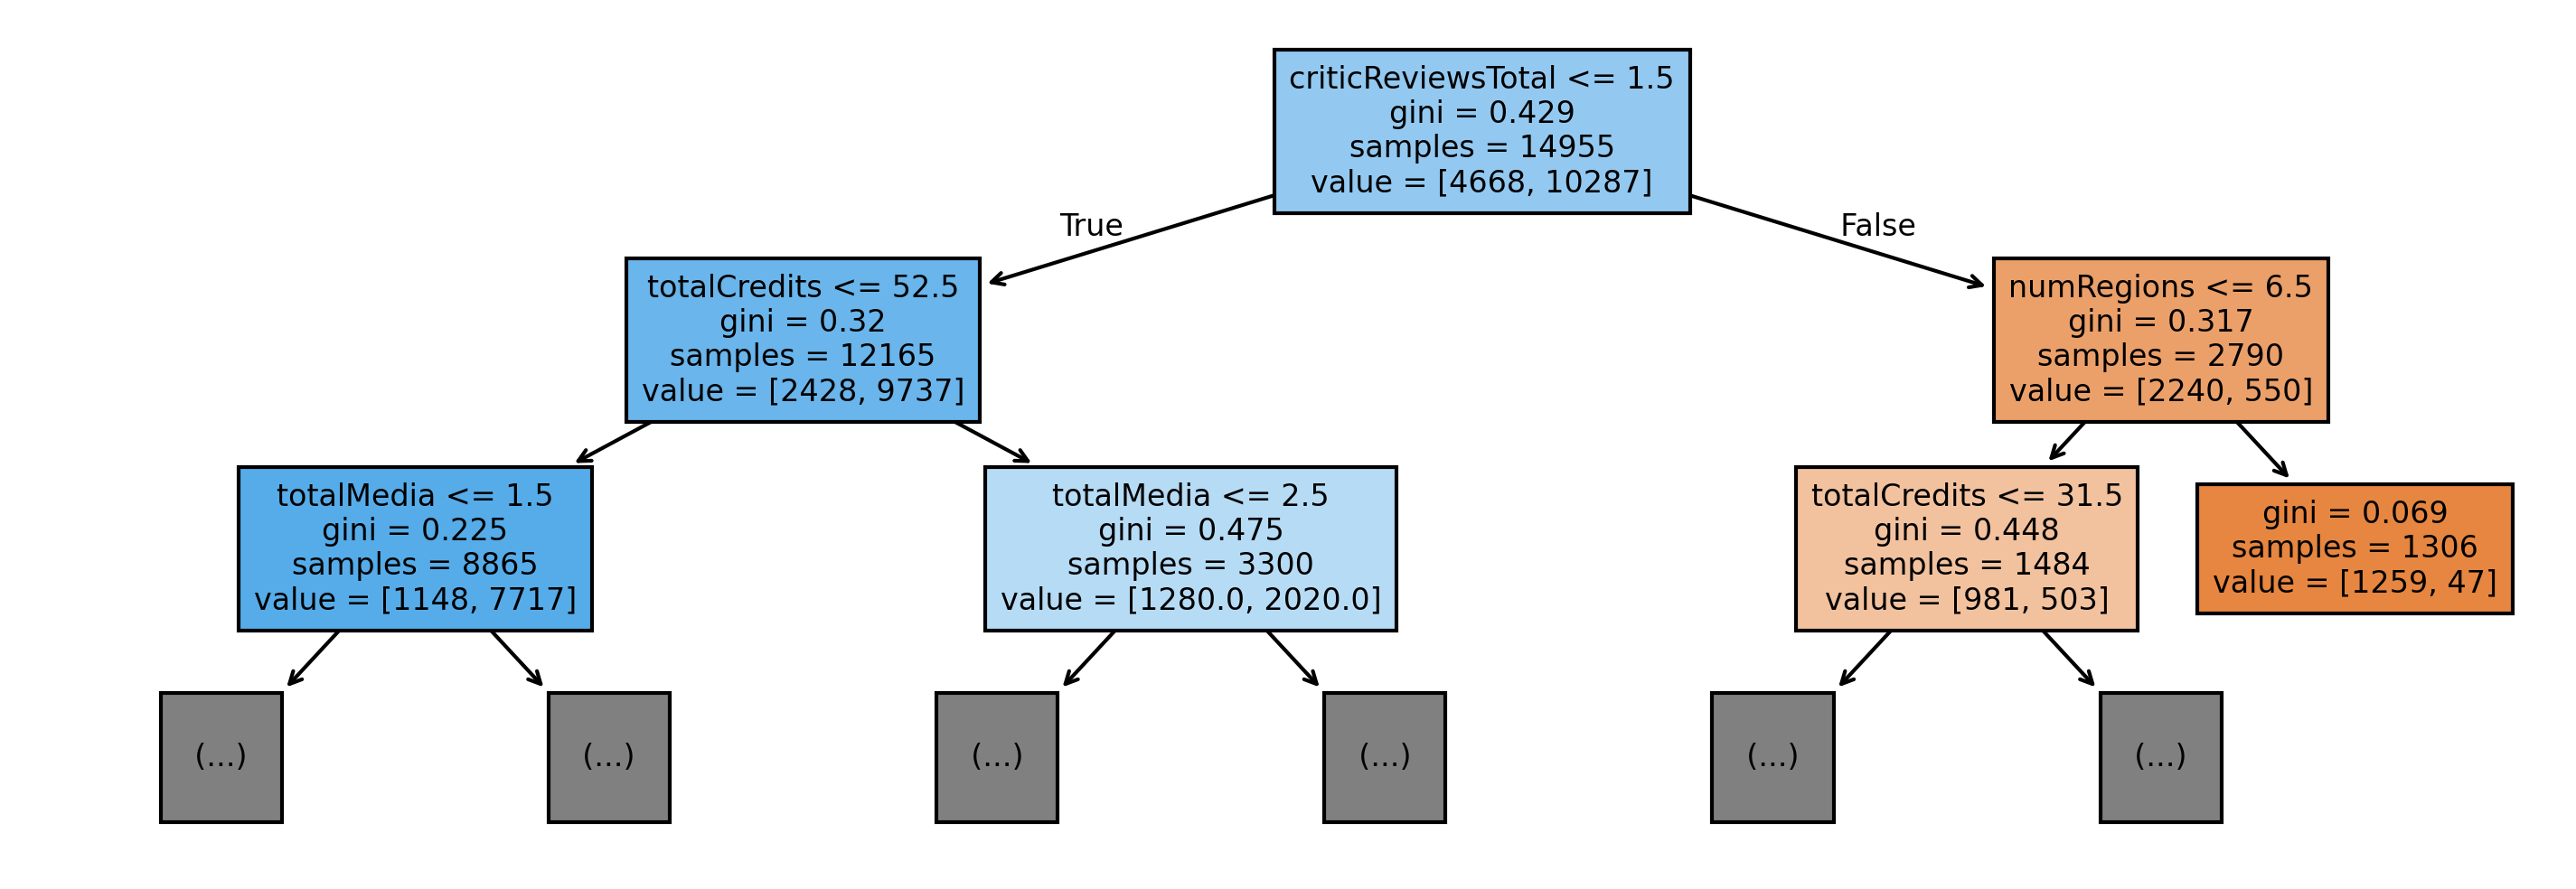
\includegraphics[width=0.8\linewidth]{plots/binary_dt.png}
    \captionsetup{justification=centering, width=0.9\linewidth}
    \caption{Decision Tree for binary classification}
    \label{fig:binary_dt}
\end{figure}

Unsurprisingly, the most important feature for the model was \texttt{criticReviewsTotal},
which amounted to 0.6 in the feature importance ranking. The following other 3 more important
features were \texttt{totalCredits} (0.15), \texttt{totalMedia} (0.10) and \texttt{numRegions} (0.09).
These four features take up around 93\% of the total feature importance, and are all present in the first
two splits shown in the Decision Tree.\\
% Classification performance is summarized in Table~\ref{tab:binary_classification_report}.

% \begin{table}[H]
%     \centering
%     \begin{tabular}{lcccc}
%         \toprule
%         \bf{Class} & \bf{Precision} & \bf{Recall} & \bf{F1-score} & \bf{Support} \\
%         \midrule
%         \bf{Low engagement} & 0.86 & 0.90 & 0.88 & 3416 \\
%         \bf{High engagement} & 0.75 & 0.69 & 0.72 & 1561 \\
%         \midrule
%         \bf{Macro avg} & 0.81 & 0.79 & 0.80 & \\
%         \bf{Weighted avg} & 0.83 & 0.83 & 0.83 & \\
%         \midrule
%         % & & \textbf{Train} & \textbf{Test} & \\
%         % \midrule
%         \bf{ROC AUC} & & & 0.87 & \\
%         \bf{Accuracy}  &  & & 0.83 & \\
%         \bottomrule
%     \end{tabular}
%     \caption{Classification report for binary classification}
%     \label{tab:binary_classification_report}
% \end{table}
Train performance was overall similar to the test performance; in particular, the respective accuracies
were of 0.83 and 0.84, and macro-F1 scores were 0.82 and 0.80.
In any case, post-pruning was tested, but did not yield any performance improvement, and was therefore
not applied.
The \textit{High Engagement} class showed low Recall values (0.71 on train set, 0.68 on test set).
This might be a consequence of class imbalance, as well as poor separability of the two classes.
This assumption is further supported by the
Precision scores of the class (0.78 on train, 0.75 on test).

% \begin{figure}[H]
%     \begin{minipage}{0.58\textwidth}
        % Figure~\ref{fig:conf_matr_binary_dt} shows the confusion matrix for the obtained
        % Decision Tree, with results regarding the test set.
        % As can be seen, a significant number of \textit{High Engagement} records was misclassified,
        % leading to a low Recall for that class.
        % This might be a consequence of class imbalance, as well as the possible presence
        % of noise in the data. It's also possible that the two classes are not well separated, leading
        % the model to prioritize the predominant class.\\
%     \end{minipage}
%     \hfill
%     \begin{minipage}{0.38\textwidth}
%         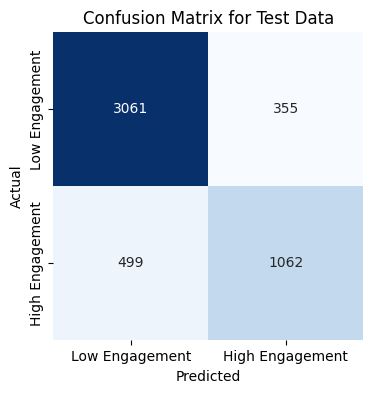
\includegraphics[width=\linewidth]{plots/binary_dt_confusion_matrix.png}
%         \captionsetup{justification=centering, width=0.9\linewidth}
%         \caption{Confusion matrix for binary classification}
%         \label{fig:conf_matr_binary_dt}
%     \end{minipage}
% \end{figure}

\subsection{Model Comparison}

\section{Multiclass classification}\label{sec:multiclass_classification}
Among the multiclass features in the training set, \texttt{titleType} was selected as the target variable
for this task, due to its relevance within the dataset. Because of their strong correlation with
\texttt{titleType}, the feature \texttt{canHaveEpisodes} and the genre \textit{Short} were excluded from the
feature set. Furthermore, since the primary imputation method for missing values in \texttt{runtimeMinutes}
relied on information from the target variable, these values were re-imputed to avoid data leakage.
Specifically, missing entries were filled by sampling from the overall distribution of
\texttt{runtimeMinutes}, without referencing \texttt{titleType}.\\

One final point to note is the imbalance in the target feature (previously shown in
figure~\ref{fig:titleType_distrib}), which was explicitly taken into account
during the design of the models. As for the binary classification task, macro-averaged F1-score was
a key metric for model evaluation, as it provides a balance between each class's precision and recall.



% This feature was created to impute the missing values of the original \texttt{runtimeMinutes} variable,
% but without using the median value according to the titleType. Instead, the missing values were imputed using the help of two variables: \texttt{canHaveEpisodes} and \texttt{is\_Short}
% (as one of the resulting variables of the multi-label one-hot encoding process of the \texttt{genres} attribute).
% In particular, 
% \textbf{SCRIVERE COME E' STATA IMPUTATA NO\_TT - con canhaveepisodes e is\_short preso dai generi}.
% This approach prevents a significant error, as it would be methodologically incorrect to use \texttt{titleType}-based 
% imputation for an attribute when \texttt{titleType} itself is the target variable to predict.
\subsection{K-NN}
\subsection{Naïve Bayes}
\subsection{Decision Trees}
Like for the binary classification task, the Decision Tree model was trained without normalizing or
transforming the features, making the model more interpretable. Feature selection was performed by studying
feature importance, while hyperparameters were optimized with a Randomized Search,
which used Repeated Stratified 5-Fold Cross-Validation with 5 repeats on the training set, optimized for
the macro-averaged F1-score.
The best configuration found used Entropy as splitting criterion, had a max depth of 14, a minimum of
5 samples per leaf, and a minimum of 8 samples in order to split an internal node.
\begin{figure}[H]
    \centering
    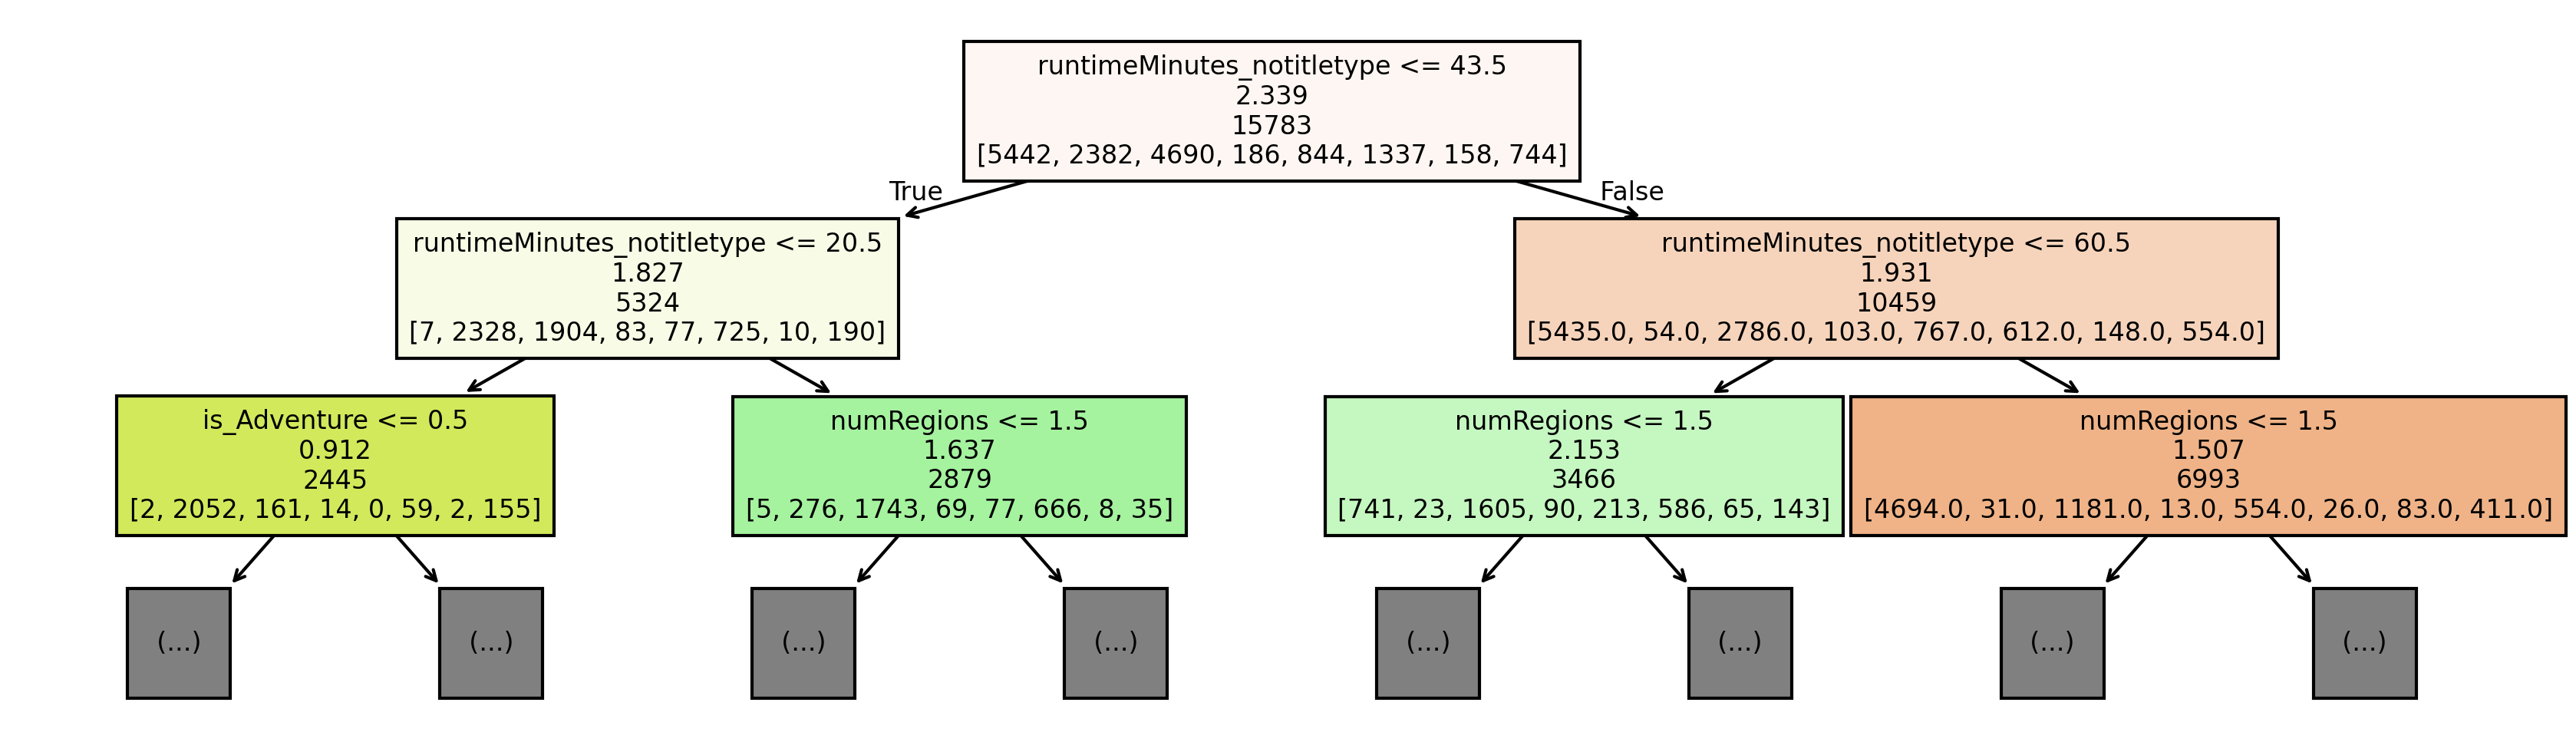
\includegraphics[width=0.88\linewidth]{plots/multiclass_tree.png}
    \captionsetup{justification=centering, width=0.9\linewidth}
    \caption{Decision Tree for multiclass classification}
    \label{fig:multiclass_dt}
\end{figure}

\begin{wrapfigure}{r}{0.45\textwidth}
    \centering
    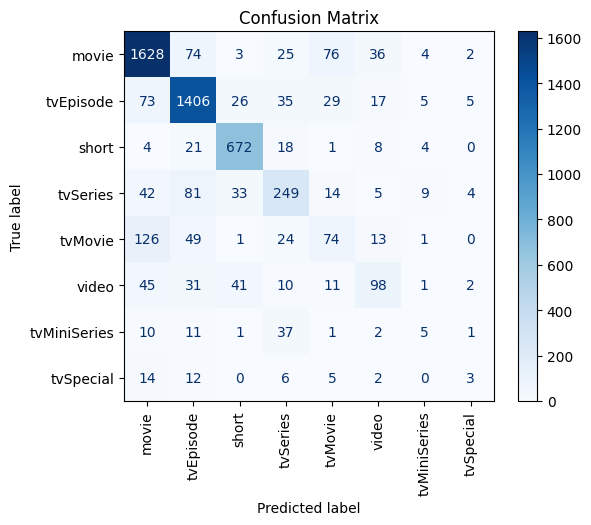
\includegraphics[width=0.48\textwidth]{plots/multiclass_dt_conf_matrix.png}
    \caption{Confusion matrix for the model}
    \label{fig:multiclass_dt_conf_matrix}
\end{wrapfigure}
Figure~\ref{fig:multiclass_dt} shows the Decision Tree obtained for the multiclass classification task.
The most important feature for the model was\texttt{runtimeMinutes}, on which the first two levels
of the tree are based, with a feature importance of 0.45.
Three out of the four splits in the following level are based on \texttt{numRegions} being smaller than
2, giving the feature an importance of 0.13; the fourth is based on the \textit{Adventure} genre,
which has an importance of 0.01.
The model showed a general tendency towards overfitting, and many configurations were tested to prevent
this.
The overall accuracy shows a significant drop (from 0.86 on the train set, to 0.75 on the test set),
as well the macro-averaged F1-score, going from 0.65 to 0.52.
This was given from the \textit{tvMiniSeries} and \textit{tvSpecial} classes: these had f1-scores of
0.35, 0.22 respectively on the train set, and both had 0.10 on the test set. Since they were by far
the least represented classes, they required a trade-off between low-represented classes classification
and generalization. This can be seen in figure~\ref{fig:multiclass_dt_conf_matrix}, which shows the fact
that most predictions for these classes were misclassified.
In order to mitigate this, post-pruning was tested, but did not give particular benefits.
Higher values for the parameter $\alpha$ had minor positive effects on the generalization
capabilities of the models, at the cost of losing predictions on the less represented classes.
Another aspect highlighted by the confusion matrix is the fact that \textit{tvMovie} was often
classified as \textit{movie}, leading to a Recall value of 0.26 on the test set.
This is likely due to the fact that the two classes are overlapping, since they are semantically related,
and is further supported by the fact that the most common misclassification for \textit{movie} was
\textit{tvMovie}, albeit with a low number of occurrences, likely due to it being the biggest class.
A similar case can be made for \textit{tvSeries} and \textit{tvMiniSeries}, with 37 out of the total 68
of the \textit{tvMiniSeries} records being misclassified as \textit{tvSeries}.



\subsection{Model Comparison}
Because of class imbalance, for evaluation purposes,
macro-averaged F1-score was heavily considered. %classification

\chapter{Regression}
\label{ch:capitolo4}
Different regression techniques were applied to the dataset, testing
on different combinations of attributes. The target variable chosen for
Univariate and Multiple regression was \texttt{criticReviewsTotal}, while
for Multivariate regression, the target variables were both
\texttt{userReviewsTotal} and \texttt{criticReviewsTotal}.


\section{Univariate and Multiple Regression}
For Univariate Regression, the attribute
\texttt{criticReviewsTotal} was chosen
as the target variable. This choice was made because it has a high correlation
with the attribute \texttt{userReviewsTotal}, allowing univariate regression
to be performed, while maintaining a clear separate semantic meaning.
For Multiple Regression, the target variable was kept the same, in order to
allow for a direct comparison of the results obtained with the two techniques.
The feature also has an important semantic meaning, strictly related to the
engagement towards the product, which links this analysis to the binary
classification performed in section~\ref{sec:binary_classification}.

\section{Multivariate Regression}
 %regression

\chapter{Pattern Mining}
\label{ch:capitolo2}
To perform this task, continuous attributes were discretized based on their distributions, 
aiming for bins that were both semantically meaningful and reasonably balanced in size. 
The selected numerical attributes (not normalized) for the pattern mining task, along with their binning, are:
\begin{table}[h]
\centering
\begin{tabular}{ll}
\toprule
\textbf{Attribute} & \textbf{Binning} \\
\midrule
\texttt{runtimeMinutes} & VeryLowRTM (1-30), LowRTM (31-60), MediumRTM (61-90), HighRTM (91-220) \\
\texttt{rating} & VeryLowR (1-3), LowR (4-6), MediumR (7), HighR (8), VeryHighR (9-10) \\
\texttt{totalCredits} & VeryLowC (0-15), LowC (16-35), MediumC (36-65), HighC (66-15742) \\
\bottomrule
\end{tabular}
\caption{Binning of the continuous attributes}
\end{table}\\
Regarding discrete attributes, \texttt{titleType} was considered for this task, kept in its original form. 
On the other hand, the values of each of the 7 attributes \texttt{countryOfOrigin\_[continent code]}\footnote{see subsection 1.1.3 for the list of the features} were binarized into:
\begin{itemize}
    \item \texttt{not\_from\_[continent code]}: when the value of the attribute is 0
    \item \texttt{is\_from\_[continent code]}: when the value of the attribute is $\geq$ 1
\end{itemize}
Binarization was preferred over creation of multiple bins, as it allows for a more linear interpretation of the results. 
An attempt was performed to include genres; however, this did not lead to more interesting results.

\section{Extraction and discussion of frequent patterns}\label{sec:freq_patterns}
\begin{figure}[H]
    \centering
    % First subfigure
    \begin{subfigure}{0.49\textwidth}
        \centering
        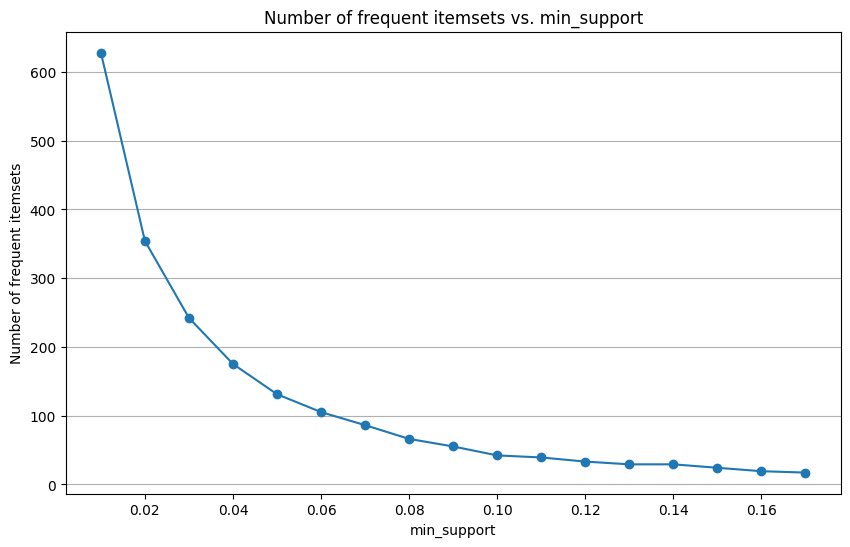
\includegraphics[width=0.98\textwidth]{plots/5_min_sup.png}     %se teniamo 0.65 ci sta sotto la tabella delle continuous
        \caption{Plot of frequent itemsets with varying \textit{support}}
        \captionsetup{width=0.9\linewidth, justification=centering}
        \label{fig:min_sup}
    \end{subfigure}
    \begin{subfigure}{0.49\textwidth}
        \centering
        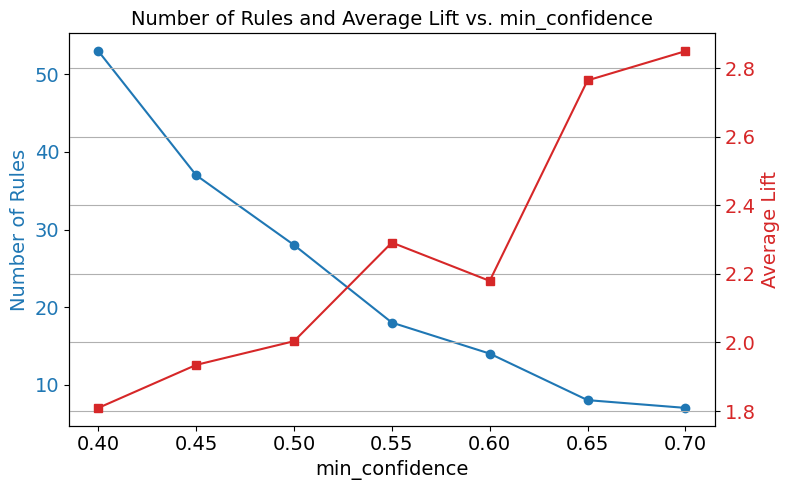
\includegraphics[width=0.98\textwidth]{plots/5_min_conf.png}     %se teniamo 0.65 ci sta sotto la tabella delle continuous
        \caption{Plot of lift and number of rules with varying \textit{confidence}}
        \captionsetup{width=0.9\linewidth, justification=centering}
        \label{fig:min_conf}
    \end{subfigure}
    \captionsetup{justification=centering}
    \caption{Plots of minimum support and confidence - \textit{Apriori} algorithm}
    \label{fig:distrib}
\end{figure}
\textit{Apriori} was the algorithm chosen to extract frequent patterns. 
Figure~\ref{fig:min_sup} shows how the number of frequent itemsets changes with support values ranging from 0.01 to 0.18. 
The curve of the plot begins to flatten between 0.08 and 0.1, so a support value of 0.08 was selected, resulting in 66 frequent patterns.\\

It is interesting to observe the top frequent itemsets of size 1, 2, and 3, as shown in Table~\ref{tab:top-itemsets}. 
From the itemset of size 1 it was noticed that approximately 48.5\% of the objects in the dataset are from North America, highlighting the prevalence of this region.

\begin{minipage}{0.42\textwidth}
The size-2 itemset reveals that 1/4 of the objects is both from North America and has a very low runtime.
This pattern becomes more specific in the top size-3 itemset, where almost 10\% of the data corresponds to TV episodes with both characteristics.
\end{minipage}
\hfill
\begin{minipage}{0.56\textwidth}
\centering
\begin{tabular}{ccl}
\toprule
\textbf{Size} & \textbf{Support} & \textbf{Itemsets} \\
\midrule
1 & 0.485 & (is\_from\_NA) \\
2 & 0.204 & (VeryLowRTM, is\_from\_NA) \\
3 & 0.094 & (tvEpisode, VeryLowRTM, is\_from\_NA) \\
\bottomrule
\end{tabular}
\captionof{table}{Top itemsets of sizes 1, 2, and 3}
\label{tab:top-itemsets}
\end{minipage}


% It is interesting to observe the top frequent itemsets of size 1, 2, and 3, as shown in Table 5.2. 
% From the itemset of size 1 it was noticed that approximately 48.5\% of the objects in the dataset are from North America, highlighting the prevalence of this region. 
% The size-2 itemset reveals that 1/4 of the objects is both from North America and has a very low runtime. 
% This pattern becomes more specific in the top size-3 itemset, where almost 10\% of the data corresponds to tv episodes with both characteristics.

% \begin{table}[h]
% \centering
% \begin{tabular}{ccl}
% \toprule
% \textbf{Size} & \textbf{Support} & \textbf{Itemsets} \\
% \midrule
% 1 & 0.485 & (is\_from\_NA) \\
% 2 & 0.204 & (VeryLowRTM, is\_from\_NA) \\
% 3 & 0.094 & (tvEpisode, VeryLowRtm, is\_from\_NA) \\
% \bottomrule
% \end{tabular}
% \caption{Top Itemsets of 1, 2, 3 sizes}
% \end{table}



\section{Extraction of rules}\label{sec:rules}
After extracting the frequent patterns, association rules were generated.
To find a value of \textit{confidence} that balances the number of rules and their strength (measured with \textit{lift}), 
the plot in Figure\ref{fig:min_conf} was analysed. A \texttt{min\_confidence} of 0.55 was selected, guaranteeing an average \textit{lift} of 2.3 and 
a significant number of rules, i.e. 18. The top 10 rules extracted (ranked by lift) are:
\begin{table}[h]
\centering
\begin{tabular}{cllcccccc}
\toprule
\textbf{Rule} & \textbf{Antecedents} & \textbf{Consequents} & \shortstack{\textbf{Ant.}\\\textbf{Sup.}} & \shortstack{\textbf{Cons.}\\\textbf{Sup.}} & \textbf{Sup.} & \textbf{Conf.} & \textbf{Lift} \\
\midrule
0 & (short) & (VeryLowC, VeryLowRTM) & 0.160 & 0.128 & 0.093 & 0.583 & 4.568 \\
1 & (VeryLowC, VeryLowRTM) & (short) & 0.128 & 0.160 & 0.093 & 0.731 & 4.568 \\
2 & (HighRTM) & (movie) & 0.177 & 0.319 & 0.154 & 0.866 & 2.719 \\
3 & (is\_from\_NA, short) & (VeryLowRTM) & 0.082 & 0.375 & 0.082 & 0.995 & 2.654 \\
4 & (VeryLowC, short) & (VeryLowRTM) & 0.094 & 0.375 & 0.093 & 0.994 & 2.650 \\
5 & (short) & (VeryLowRTM) & 0.160 & 0.375 & 0.159 & 0.993 & 2.648 \\
6 & (VeryLowRTM, short) & (VeryLowC) & 0.159 & 0.234 & 0.093 & 0.588 & 2.513 \\
7 & (short) & (VeryLowC) & 0.160 & 0.234 & 0.094 & 0.587 & 2.511 \\
8 & (is\_from\_NA, LowRTM) & (tvEpisode) & 0.121 & 0.303 & 0.090 & 0.742 & 2.447 \\
9 & (MediumRTM) & (movie) & 0.229 & 0.319 & 0.165 & 0.720 & 2.260 \\
\bottomrule
\end{tabular}
\caption{Top 10 rules extracted with \textit{Apriori} (ranked by lift)}
\end{table}


\section{Exploiting rules for target prediction}\label{sec:prediction_rules}
One way to exploit the previously extracted rules is for target prediction. 
Firstly, rules with \texttt{VeryLowC} as target (rows 6 and 7 in the Table 5.3), show that short contents with very low runtime are highly likely to be associated with very low credits, 
probably reflecting the involvement of a limited production or cast. 
Both rules show a strong association, with a \textit{lift} greater than 2.5, with the more specific one (VeryLowRTM and short) offering a better potential for targeted prediction. \\

The target \texttt{is\_from\_NA} was then analysed to find the antecedents (as shown in Table 5.4), that increase the likelihood of an object of 
being from North America. Even though the \textit{lift} value of those rules is below average, these rules were still considered, due to their meaningful interpretability.
The analysis suggests that North American origin is associated with TV episodes, shorter durations, and high ratings or numerous production credits.
\begin{table}[h]
\centering
\begin{tabular}{cllcccccc}
\toprule
\textbf{Rule} & \textbf{Antecedents} & \textbf{Consequents} & \shortstack{\textbf{Ant.}\\\textbf{Sup.}} & \shortstack{\textbf{Cons.}\\\textbf{Sup.}} & \textbf{Sup.} & \textbf{Conf.} & \textbf{Lift} \\
\midrule 
12 & (HighR, tvEpisode) & (is\_from\_NA) & 0.144 & 0.485 & 0.092 & 0.639 & 1.317 \\
13 & (HighC) & (is\_from\_NA) & 0.152 & 0.485 & 0.156 & 0.627 & 1.292 \\
14 & (tvEpisode, LowRTM) & (is\_from\_NA) & 0.144 & 0.485 & 0.090 & 0.624 & 1.285 \\
15 & (tvEpisode) & (is\_from\_NA) & 0.303 & 0.485 & 0.186 & 0.612 & 1.261 \\
16 & (tvEpisode, VeryLowRTM) & (is\_from\_NA) & 0.153 & 0.485 & 0.093 & 0.611 & 1.259 \\
17 & (LowRTM) & (is\_from\_NA) & 0.219 & 0.485 & 0.121 & 0.553 & 1.139 \\
\bottomrule
\end{tabular}
\caption{\texttt{is\_from\_NA} as target}
\end{table}
 %pattern mining


% \thispagestyle{empty}
\clearpage

%\listoffigures secondo me non utile
% \thispagestyle{empty}

\printbibliography
%\renewcommand{\listfigurename}{List of figures}
%\listoffigures

\end{document}
